\chapter{Methods\label{Methods}}

This chapter deals with the design of our system, an overview of the
implementation and technical aspects on the data that we work with. We
will be taking a look at how the first prototype was designed and how
it branched out to several different versions due to experiments with
various heuristics applied to the data. We will go through the
individual modules of the system and how they communicate through the
data formats. After giving a thorough description on the data we work
with in the system, we finally round off the chapter with some of the
technical conclusions that we got from building the system.

\section{System Overview and Design\label{SystemOverviewAndDesign}}

In this section, we lay out the design of the system. In section
\ref{FirstPrototype}, we describe how the first prototype is put
together while in section \ref{DiseaseMatrix}, we describe the
different ways we have tried to structure the system. Finally, in section
\ref{FilteringMatrix}, we mention how the applied filters have led to
several different versions of the matrices that make up the heart of
the system. For full overview see figure \ref{OverviewDiagram}

\subsection{The First Prototype\label{FirstPrototype}}

We have made a modular design that is divided into five major
components representing our system. The first module is a web crawler
called \textit{DiseaseCrawler}. It gathers preliminary data from
Rarediseases.info and saves it in a specified data format on the disk
(see section \ref{Crawler}), allowing the next module to read it in
and process it. \textit{The Search and Information Retrieval} (SIR)
module searches and retrieves MedLine records from PubMed.org in
accordance to the data gathered in the crawler module. SIR saves its
data in a file under the disease name, containing up 500 MedLine
records per disease-search and a description if one is found (see
section \ref{SIR}). This allows the third module \textit{TermDoc} to
read in the data, convert all the disease to sub term document
matrices and construct a large term document matrix from the data from
the sub-matrices, saving the term document matrix in Matrix Market
format (see section \ref{MatrixMarket}). As an option one can include a filter
just before the construction of the large term document matrix (or on
the sub-matrices), e.g. a stemmer and/or stop word remover or other
kinds of filters, like log-transformation of the term counts and the
much used term frequency - inverse document frequency (TF-IDF). The
resulting data from the TermDoc module can now be used for
querying. This is done through the \textit{QueryInterface} module that
implements the cosine measure to perform correlation between vectors,
i.e. between a query vector and a document vector in our term document
matrix. To be able to give a disease name instead of just a MedLine
record, we need to score the disease in relation to the given query
vector. This is done by a consensus method, where we select the number
of MedLine records to use a basis of the consensus so that each
MedLine record has one or more disease names attached to it (the same
MedLine record can be returned from different diseases). We then sum
the score from each MedLine record under the given disease names
and sort the total scores. Those with the highest total score have the
greatest correlation with the search query, and therefore these are the
most likely to be our disease.

The modular design of the prototype system allows the different
modules to be replaced with more efficient modules or modules that
gather data from different sources - as long as the new module
conforms to the specified data formats. It allows for an easy addition
of new heuristics and filtering modules to specific points in the data
modelling.

\subsection{Branching the Prototype\label{DiseaseMatrix}}

A major branch in our design sprung when we realised the potential of
building a disease matrix instead of a term document. Though severely
simplifying our data, this model is a reduced version of the term
document matrix and is a lot easier and faster to work with.

The disease matrix is based on the same data as the term document
matrix. It differs in the way that it contains all the information
that we have about each disease from the MedLine records, summed into
one vector describing the disease. The new disease matrix still needs to
contain the same terms as the term document matrix but is now made of
a disease vectors instead of document vectors. This makes the
individual disease vector less sparse than a document vector. The same
preprocessing options that run on the term document matrix, can be
applied to the disease matrix just as easily.

\subsection{Filtering for New Matrices\label{FilteringMatrix}}

Adding filters to the prototype system spawns new matrices to work on
(as shown on in the figure below \ref{OverviewDiagram}). The
sub-matrices generated from the MedLine records are generated both as
stemmed and non-stemmed. From these, two large term document matrices
and two different disease matrices are generated. Adding another heuristic, the
large matrices are TF-IDF transformed (with and without
normalization).

Yet another pool of sub-matrices are created by SVD and dimensionality
reduction, leading to yet another large disease matrix to perform
tests and potential keyword extractions on.

Again we mention that filters and heuristics should be pretty easy to
add since only the data formats in between the modules needs to be
kept in order.

\begin{figure}[H]
        \begin{center}
          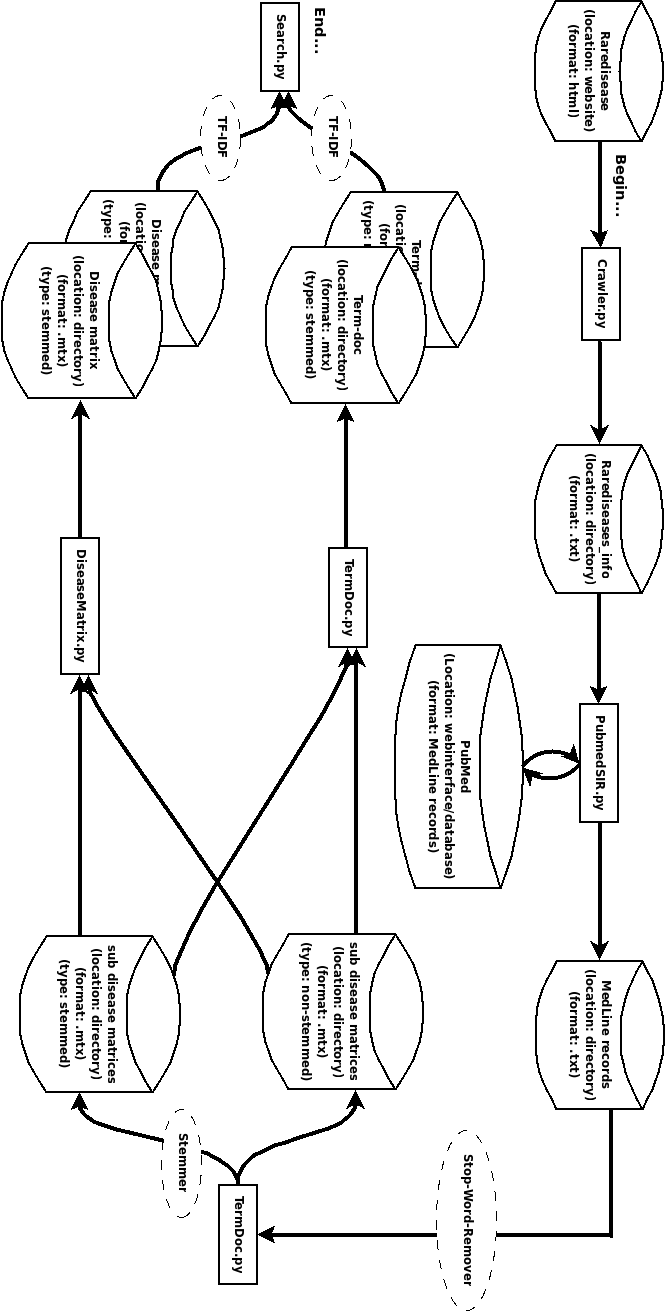
\includegraphics[width=0.8\textwidth]{diagrammer/system_overview_rotate.png}
        \end{center}
        \caption{Overview diagram of the system}
        \label{OverviewDiagram}
\end{figure}

\section{Modules}

In this section, we will go through the individual modules described
in section \ref{SystemOverviewAndDesign}. We will provide an
overview of the module, its parts and the way that the data --- in
between the modules --- is structured. We will also be looking at the
filter modules, the auxiliary modules and the modules used for data
analysis.

\subsection{Crawler\label{Crawler}}

\subsubsection{Overview and Purpose}
The crawler is the first step in creating a database of MedLine
records, containing information about rare diseases, since its main
purpose is to gather information about what to search for in PubMed.

As described in \ref{Rarediseases_info}, Raredisease.info contains a
list of rare diseases and a varying degree of information on each
specific disease. We were referred to the website by Henrik L.  J\o
rgensen \cite{TheDude}. A Crawler to collect information from the
site, was the first module to be made. The crawler goes through every
disease from A to Z and 0-49 and saves the names of the diseases and
(if any exist) the synonyms, the specialized search string for PubMed
and a description of the disease. This information is then used by a
SIR-module which is described in the following section \ref{SIR}.

Our main module is named \textit{DiseaseCrawler}. It crawls the
Rarediseases.info web page and gathers information as described
above. It is a rather large module since it has to take a series of
anomalies into account when crawling Rarediseases.info (like
dysfunctional sub pages, strange characters and unexpected
white-spaces). It utilizes the auxiliary modules \textit{TextCleaner}
and \textit{IOmodule}, described in section \ref{AuxModules}.


\subsubsection{Methods and data description}
The crawler accepts a list of letters for which to gather information
from, e.g. ['A'] means gather all diseases beginning with A. It
utilizes the HTML parser library Beautifulsoup \cite{BS} to parse the
web pages, looking for disease names, synonyms, handcrafted searches
and uids. The crawled data is all stored in database of dictionaries
on the form:

\begin{center}
{\small
\{'terms': '', 'desc': '', 'db': u'omim', 'syn': [u'Pectus excavatum', u' macrocephaly and dysplastic nails', u'Familial short stature', u' developmental delay', u' pectus abnormalities', u' distinctive facies', u' and dysplastic nails'], 'uid': u'600399'\} 
}
\end{center}

The name of the file --- that each of the data sets are stored in ---
is the name of the disease. The above shows a example for the disease
'Zori Stalker Williams syndrome'. The key 'terms' will contain the
handcrafted search string for PubMed if one is found while 'desc'
contains the description of the disease if one is available
(unfortunately on Rarediseases.info only 6.94\% contain one). 'db'
represents the choice of database to use and refers to either PubMed
or OMIM in our current cases. It is necessary to know how to search for
the disease in Entrez, as described in the following section. 'syn' is
a list containing the various synonyms associated with the disease and
used for finding more relevant information about the disease. 'uid' is
a unique identifier found on all OMIM links and in some cases on
pre-calculated PubMed searches.

\subsection{SIR (Search and Information Retrieval)\label{SIR}}

\subsubsection{Overview and Purpose}
The \textit{PubMedSIR}-module reads in the information saved by the crawler (or any
other crawler). It uses Entrez for accessing, searching and retrieving
MedLine records from PubMed. The information contained within the
MedLine record represents our knowledge base about the diseases. The
\textit{PubMedSIR}-module is set to search in such a way that we hope to optimizes
the retrieval of records that are actually relevant to the given disease. A
maximum of 500 MedLine records are downloaded per disease using a two
phase search - all containing an abstract.

The main module is called \textit{PubMedSIR} and is used to search and
retrieve MedLine records from the PubMed database.

As mentioned above the searching is split into two phases, where at
 most 250 MedLine records are looked for in each phase. It first examines
whether there is a handcrafted search string to search for or whether
the disease has a PubMed or OMIM unique-id (uid). When searching for
the handcrafted search string, \textit{PubMedSIR} automatically adds the
additional search options ``AND hasabstract[text]'' to the string. This
makes sure that all the MedLine records, that are returned, contain
an abstract. This is unfortunately not possible when dealing with
PubMed/OMIM uids which means that we have to employ other means to
ensure that the returned MedLine records contain an abstract. This is
carried out by the method \texttt{getMedLineList} which takes a list of
PMIDs, downloads them from PubMed and runs through all the MedLine
records, selecting only those containing an abstract. Making a local
clean to ensure that the MedLine records contain abstracts also
means that we can not guarantee 500 MedLine abstracts for a disease
even thought they are available. This is a minor fault in our system
that should have been corrected if time allowed it but we have chosen
to continue with the information we have available. Alternatively
additional search options could be to also include constraints for
getting only abstracts in English, only records published after a
certain date etc. For options see the site PubMed help search
\cite{PubMedHelpSearch}

\textit{PubMedSIR} relies primarily on the function
\texttt{getArticleIDsFromMultipleSources} for searching across the two
major databases of Entrez - PubMed and OMIM. We have chosen not to
remove duplicate MedLine records between the first and second phase of
the search because it is our belief that --- if a record is present in
both searches --- the terms are worth counting twice. The searches are
done as the described below.

First phase of the search:
\begin{itemize}

\item Search for term if it is present, OR

\item Search for PubMed/omim uid.

\item If we have obtained less than 250 MedLine records,
  
\begin{itemize}

  \item Search for the disease name on PubMed.

  \item Eliminate duplicates.

  \end{itemize}
\end{itemize}

Second phase of the search:
\begin{itemize}

\item Calculate all possible combinations of the synonyms.

\item Search for the combined synonym. If a combination returns 0
  results then eliminate all future searches that contains this
  combination since PubMed put 'AND' in between search terms (meaning
  that future searches containing this combination will also return 0
  results).

\item Fill up until we get at most 500 MedLine records.

\end{itemize}

\subsubsection{Method and data description}
The primary function of the module is \texttt{gatherOfAllThings},
which reads in the information that was saved by the crawler. This
information is passed onto \texttt{getArticleIDs} that in turn calls
\texttt{getArticleIDsFromMultiSource} which searches the items
specified within the disease dictionary. \texttt{getArticleIDs} is
also the function that keeps track of the number of MedLine records
that are downloaded for each disease.

A typical dictionary read in from the crawler looks as follows:

\begin{center}
{\small
\{'disease x': \{'syn' : [xx, yy, zz], 'term' : string, 'uid' : string,
    'description' : string, 'db' : pubmed|omim\}, 'disease y': \{'syn' :
    [aa, bb], 'term' : string, 'uid' : string, 'description' : string,
    'db' : pubmed|omim\}, ...\}
}
\end{center}

\texttt{gatherOfAllThings} completes by performing a write out of the
MedLine records to the disk in the following format:

\begin{center}
{\small
\{'disease a': [pmid1, pmid2, pmid3...], 'disease b' : [pmidx,
    pmidy,...], ...\}
}
\end{center}

The \textit{PubMedSIR} module uses the following auxiliary modules
(see section\ref{AuxModules}):

\begin{itemize}
\item \textit{SearchTermCombiner} which is a simple module that is
  used to combine search terms in all possible unique
  combinations.
\item \textit{IOmodule} handles Input/Output.
\item \textit{TextCleaner} is used to sanitize the input strings.
\end{itemize}

For more information about the gathered data set, see section \ref{Database}.

\subsection{TermDoc\label{TermDoc}}

\subsubsection{Overview and Purpose}
The information gathered from the \textit{PubMedSIR}-module now needs
to be processed to allow queries to be made on it. An often used
method in Information Retrieval (IR) is the vector space model
\ref{VectorSpace} that represents the gathered information as document
vectors (in a term document matrix). The result is that queries to the
system can be made using a query vector, getting a similarity
score/measure against all documents contained within the model. In the
following, we will go through the creation of the sub term document
matrices, the large term document matrix and the compressed disease
matrix.

We use a two-phase approach to construct the complete term document
matrix.

In the first phase, we make a sub term document matrix for each
disease containing the information from the MedLine records. We split
up the abstract, title and MeSH terms if present. Various filters can
be applied to the terms, e.g. stemming and stop word removal. We
choose to remove any kind of punctuation and the like because
otherwise the terms remain very noisy ("blood" and "blood." would be
two different terms). We keep single letters (except for 'a' which
counts as a stop word), because many diseases contains single letters
as identification of which type they are, e.g. 'Hemoglobin C
disease'. It is an fault in our system that we do not keep 'a', but
this was discovered to late.

The second phase simply goes through the sub term document matrices
and fill the term count values into complete term document matrix.

There are two main modules. The first --- called \textit{TermDoc} --- is
able to make sub term document matrices from a folder containing
MedLine records and to combine a folder containing sub term document
matrices into a complete term document matrix. The second one is
called \textit{DiseaseMatrix} and makes a matrix with disease vectors
instead of document vectors.

\subsubsection{Method and data description}
The main function for creating the sub term document matrices from a
folder containing MedLine records is
\texttt{MedLineDir2MatrixDir}. This function requires a hash table
containing hashes for all the terms and pmids of the MedLine
record. The need for hash tables comes from the fact that the data
structures, we have chosen, do not support string entries. So hashes
can be made by the \texttt{createTermAndPmidHashes}. This function
goes through a folder containing MedLine records, while building a
term and pmid hash table. When \texttt{MedLineDir2Matrix} has read in
the hash, it proceeds by calling \textit{gatherMatrixData} on each
file within the MedLine record folder. \texttt{gatherMatrixData}
extracts information from the file by the use of the auxiliary module
\textit{RecordHandler} (see section \ref{AuxModules}). The information
can be specified by the user; title, abstract and MeSH terms are
chosen by default, as these seem to give a good overall description of
a disease. This is also the place to perform stop word removal and
stemming. We have chosen to create both a stemmed and an unstemmed
matrix in order to test what performs best. \texttt{MedLineDir2Matrix} then
calls \texttt{populateMatrix} with the data from
\texttt{gatherMatrixData}. This creates and returns a term document
matrix. Last it calls \textit{IOmodule} (see section \ref{AuxModules}) to write
the created term document matrix to the disk in Matrix Market format
(see section \ref{MatrixMarket}).

For creation of the large term document matrix, the function
\texttt{createTermDoc} is used. This goes through the folder
containing the sub term matrices and places the term count for each of
the MedLine records in the right place in the term document
matrix. This is basically done by looking up where to place them in
the hash table.  them. If the same MedLine record exists in two
different diseases, the term counts are summed. When completed, it is
written to the disk in Matrix Market format.

The disease matrix is created by calling
\texttt{constructDiseaseMatrix} with a folder of sub term document
matrices as input. It then runs through every of the sub term document
matrices and calls \texttt{getColumnSum} for each of them. This sums
the sub-matrices to a single vector and returns one row for each of
the diseases which can be used to represent it. \texttt{getColumnSum}
has the option of making the average column sum instead of just
summing them. This option can be used to normalize the disease
vectors, should it be needed. The disease matrix is (like the term
document matrix) based on hash tables. These can be created by running
\texttt{createDiseaseHash} on a folder containing sub term document
matrices.

The \textit{TermDoc} module uses the following auxiliary modules (see
section \ref{AuxModules}):

\begin{itemize}
  \item \textit{RecordHandler}, which is used for extraction with the
    records contained within the MedLine records, e.g. 'AB' for
    abstract etc.
  \item \textit{FilterInterface} used to get access to Porter stemmer
    and stop word removal of string.
  \item \textit{IOmodule} and \textit{TextCleaner} as mentioned in the
    previous section.
\end{itemize}

\subsection{FilterInterface and Heuristics}

\subsubsection{Overview and Purpose}
When dealing with the amounts of information --- in a system like this ---
there is a need to make some modifications to the data. We choose to
sanitize the input information to our system by removal of
punctuations, and by making every term lowercase. This
helps reduce the number of different terms in the system. This has the
side-effect that it also removes punctuation within description of
e.g. chromosome errors. Taking an example, the string "1q42.4-qter
duplication" will be split into '1q42', '4', 'qter' 'duplication'. We
do, however, not consider this to be a problem since the query
receives the same preprocessing as the term document matrix and it
should still be possible to retrieve the right
information\footnote{Using regular expression, it is possible to
  preserve the above string as: '1q42.4-qter', 'duplication' but we do
  not believe it important for the prototype}. The simple string
cleaning also allows the user to use other notations for the same
gene\footnote{'1q42.4-qter' and 1q42-4-qter amounts to the same}.

Another common technique in IR is to use stop word removal. This is
because words like 'this', 'the' and 'a' are very common and thereby
do not contain any information in the term-independent vector space
model. In some circumstances, it is also normal to remove single letter
characters but as some diseases are characterized by having a special
type (as mentioned in \ref{TermDoc}), we choose not to remove single
letters. However, our stop word remover does unfortunately remove 'a'
due to its frequency in the English language. As mentioned earlier, we
did not have time to correct this error.

\subsubsection{Some Numbers about Filtering}
Making a 'raw' term document matrix, without any filtering results in
1,945,966 terms. After sanitizing the information there are 465,220 terms 
and after stemming there is a further reduction to 390,766 terms.
There are a couple of modules involved with filtering. We have made a
\textit{FilterInterface} module to provide easy access to the different
filters.

\subsubsection{FilterInterface}
This is simply a gateway to various filters that are implemented in
separate modules. It is designed to return e.g. a stemmer or a stop
word remover that can be run on the abstracts before the term document
matrix is constructed. In the current prototype, it contains the
modules \textit{StopwordRemover}, \textit{Stemmer} and
\textit{TFIDFMatrix}.

\subsubsection{StopwordRemover}
The stop word remover allows for list of stop words to be supplied by
the user. By default it uses the nltk.corpus.stopwords of English stop
words which contains 127 stop words. There are other languages present
in the stop word corpus for a total of 2431 words, e.g. German,
Danish, Swedish, Norwegian and others. We do not know if any important
words are removed due in a multiple language stop word removal. We
assume that most of our information is in English and have chosen only
to remove English stop words. It is possible to setup additional
options within the \textit{PubMedSIR} module (section \ref{SIR}) so
that it will only gather MedLine records containing abstracts in
English but this is preserved for a later version of the system.

\subsubsection{Stemmer}
To preserve flexibility our system allows another stemmer to be sent
to the function replacing the default stemmer. The default stemmer is
\textit{nltk.PorterStemmer().stem} that performs stemming on our
abstract, title and MeSH terms to ``smooth'' out the terms. It is only
advisable to run the stemmer after the stop word remover. This is
mainly because the stemmer changes some stop words so that they will
not be recognised by the stop word remover, e.g. performing stemming
on 'this' results in 'thi' which is not included in the default stop
word corpus.

\subsubsection{TFIDFMatrix}
The \textit{TFIDFMatrix} module is used to perform the TF-IDF
transformation of a term document matrix using the equation from
section \ref{TFIDF}. It performs the transformation by reading the
term frequency (tf) from an original matrix only containing term
counts and then by making a log-transformation of the tf. For finding
the inverse document frequency (IDF), we have made a precalculated
hash table containing the number of documents that the different terms
are present in such that $\mathit{idf} = \frac{D}{\sum_{d\prime =
    1}\delta_{d\prime w}}$. We then store the calculation of
$\mathit{tf} \cdot \mathit{idf}$ at the term's position within the term
document matrix. The transformed term document matrix is then saved to
the disk. The module then performs normalization of the document
vector to make sure that each document has the same influence upon the
result of a query (and is used for the enhancing the speed of the
cosine similarity calculation described in section
\ref{VectorSimilarity}). The normalization is carried out as usual vector
normalization $\frac{\overrightarrow{a}}{||a||}$.

\subsection{Auxiliary modules\label{AuxModules}}

Auxiliary modules are used by the different modules to perform tasks
such as input/output, stemming, stop word removing, cleaning text string
or combining synonyms into search queries.

\subsubsection{IOmodule}
Performs various I/O functions. For instance, when a module is writing
or reading objects like hash tables to/from the disk, it simply calls
the \texttt{pickleIn} or \texttt{pickleOut} function with a path. The
object is then written or read. It is also able to return a sorted
list of file references from a folder, which is very useful when one
needs to keep track of how far the process has come. This module also
allows for term document matrices to be written or read from the disk
using the Matrix Market format (see section\ref{MatrixMarket}).

\subsubsection{TextCleaner}
This module performs string manipulation like removing tags from HTML
code, sanitizing strings for punctuation and all other special
characters, and decoding various HTML characters. Most of these task are
obtained by returning a regular expression for the specific task.

\subsubsection{RecordHandler}
The \textit{RecordHandler} module is used to read information fields
from MedLine records which it returns as a dictionary containing the
requested fields.

\subsection{SearchInterface}
The search interface implements different approaches of measuring
similarity/distance between the query vector and document vector in
our term document matrix. Our two choices of measure in the vector
space model are the cosine similarity measure and a simple sum
measure. Instead of going through all the rows (documents) in our
matrix, we take the terms from the query vector and only look up the 
the documents containing one or more of the queried terms. This limits
our search space and significantly enhances the time it takes to
process a query.

\subsubsection{SearchInterface}
This is the simple search interface that allows the different search
methods to be called, hence acting as a gateway like the
\textit{FilterInterface} described earlier.

\subsubsection{CosineMeasure}
This module is used to perform a search using the cosine measure for
distance calculations between the query vector and the rows of our
term document matrix. It uses \textit{SearchTermDoc} to get the row
indices of which rows the query terms are present in. It then sums the
scores in accordance to the occurrence of the query term. This should
resemble usual cosine measuring between vector when performed on a
pre-normalized vector space (see section \ref{VectorSimilarity}).

\subsubsection{SumMeasure}
The \textit{SumMeasure} module is used to perform a different kind of
measure. It performs a summing of the entries in the in the document
vector according to the terms of the query vector. It basically acts
as the cosine measure but is used on a vector space that is not
normalized. Again note that the reason we can compare the two measures
is because of the simplifications made in \ref{VectorSimilarity}.

\subsubsection{SearchTermDoc}
This module is used as a support module for performing searches. Given
a search vector, it will return the row indices of the term document
vectors that contain any of the terms. It can extract the term columns
with the relevant documents indices and it can create the hashes
needed for normalization and for column element counts. It is also
performs reverse look up of pmids (documents) given a pmidhash value.

\subsection{Data Analysis Tools}

In order keep track of the amount of information that we have
collected, we have made a ``crude'' module for gathering information. It
can be used to get the total number of pmids including duplicates, the
number of MedLine records containing a title or the number of diseases
that contain a description. In addition to this, we made a module to
perform hierarchical clustering of the diseases of top 20 results
returned by our system.

The modules, that are part of the data analysis suite, is
\textit{Cluster} which performs the clustering,
\textit{DistanceMeasure} which implements different
distance/similarity measures to be used within \textit{Cluster} and
\textit{Stat} which is able to count various information fields
contained within the MedLine records.

\subsubsection{Cluster}
The \textit{Cluster} module contains various functions in relation to
hierarchical clustering and drawing of dendrograms of the returned
clusters. The hierarchical clustering has unfortunately not been made
as generic as it could be. For now, slight modifications are required
between running either on a disease matrix / term document matrix or a
sub term document matrix. We have no intentions of performing a full
clustering on a term document matrix, as it simply contains too many
entries to consider clustering - at least with the resources available
currently. The hierarchical clustering and dendrogram functionality
are based on Collective Intelligence \cite{CollectiveIntelligence}
with slight modification to adopt it for our data.

\subsubsection{DistanceMeasure}
This module simply implements its own cosine measure functions for
sparse and dense matrices.

\subsubsection{Stat}
This module is able to count the various different fields within the
MedLine records, e.g. how many a title, a MeSH, etc. It is also
able to count how many duplicate pmids there are.

\section{The database\label{Database}}

Our raw data set consists mainly of two parts that are gathered
independently. The first part is the information gathered from
Rarediseases.info. The files reside in a sub folder called
\textit{rarediseases\_info} containing 6881 text files. Looking at
one of these files it is possible to see exactly what information have
been used to retrieve the MedLine records for a specific disease. The
second part of our raw data set is the information gathered from PubMed
by the \textit{PubMedSIR} module. This information can be find in the sub folder
\textit{MedLine\_records}. Again we have chosen to store it as plain
text files which enable the use of GNU unix/linux command line tools
for a quick look inside or using grep to look for specific words inside
a disease file.

Due to the limit on 500 abstracts per disease and with a total of
6,881 different rare diseases from Raredisease.info, the theoretical
upper limit on the number of abstract is 3,440,500. But since the
diseases are rare and the crawled information from Rarediseases.info
faulty at times, in reality the number of returned MedLine records is
much smaller. In fact, we only have 602,466 unique MedLine records
(about 2.8 million from the theoretical limit) and approximately
1,036,432 when counting duplicates. One of the MedLine records is even
shared among 240 diseases which indicates that it is an overview over
many diseases. There are also 505 diseases that do not return any
information at all. This means the remaining 6,376 diseases, on
average, have 94.49 MedLine records each. When searching PubMed, we
need to impose the 500-limit on the number of abstracts because (even
though the diseases are rare) some of them will return a lot of
information. Kidney cancer, though on the list of rare diseases, will
return 51,393 hits (\date{January 3, 2010}) with a search on PubMed
(only those with an abstract) and this is without considering any
synonyms or possibly handcrafted search terms.

We have chosen to remove the 505 empty disease entries from our
data set because, without any information about these diseases, our
system will be unable to find/diagnose them.

\subsubsection{More statistics on the data}
Out of the 1,036,432 MedLine records, 1,036,417 have a title. This is
nearly 100\% (99.99\%). Not all of the MedLine records have MeSH terms
although 924,026 has. This is 89.15\% of all the entries. \fxnote{This might
be a bit misleading as it count the duplicate ones too, try to get
count without duplicates.}

\section{Technical Conclusions}

When performing text mining, robustness is needed to be able to handle
various situations. This became apparent to us after having written
the first version of it. Due to the inconsistency of
Rarediseases.info, it crashed every time that it ran into a new
special case on Rarediseases.info. Therefore, when crawling website
based on incomplete topics like rare diseases, its important to carry out
proper error handling and logging which diseases were missed in the
first run as the presence of errors is almost certain. As a related side note, the
BeautifulSoup module is a really useful tool when crawling HTML since
it is able to correct and prettify many common website errors.

Gathering data from PubMed was performed by the Entrez module which on
several occasions crashed. This created the need to gather the
MedLine records in chunks to be able to resume them at any point. When
collecting data from OMIM- or PubMed-uid links, there is no way to
ensure that the returned MedLine records contains abstract and this
needs to be dealt with locally (as mentioned in \ref{SIR}). Before
performing text or data mining, ALWAYS seek the permission of those
running the site or sites. During this project, we got banned from
Rarediseases.info once and from Orpha.net twice. This was not because
we broke any laws or rules but because most websites today protects
themselves from harmful bots, replay attacks and other risks to the
website. If you do not have permission to find information on the
website, at least make sure you give your credentials, browser type,
etc. with the crawler.

Constructing a term document matrix requires a sparse data structure
for being stored on disk and in memory but when working with document
vectors, making them dense can give a huge speed up on arithmetic
operations. Choosing to rewrite some of the more computational parts
to a low level language like C would also increase performance. Saving
intermediate steps along the way while making term document matrices
also allows other preprocessing steps to be performed, if needed later
in the project and is recommendable for large projects.

When querying the matrices, it is important to try several different
methods since the most well known or obvious one, might not be the
best choice (as we shall see in the following chapter).
